%Where we previously assumed the existence of an ideal payment procedure, we now
%describe the concrete technical construction for the moneTor payment scheme.

\subsection{Economic considerations}

% A schematic of the cash
%flow cycle is illustrated in Figure~\ref{fig:economic}.

%\begin{figure}[h] \centering
%  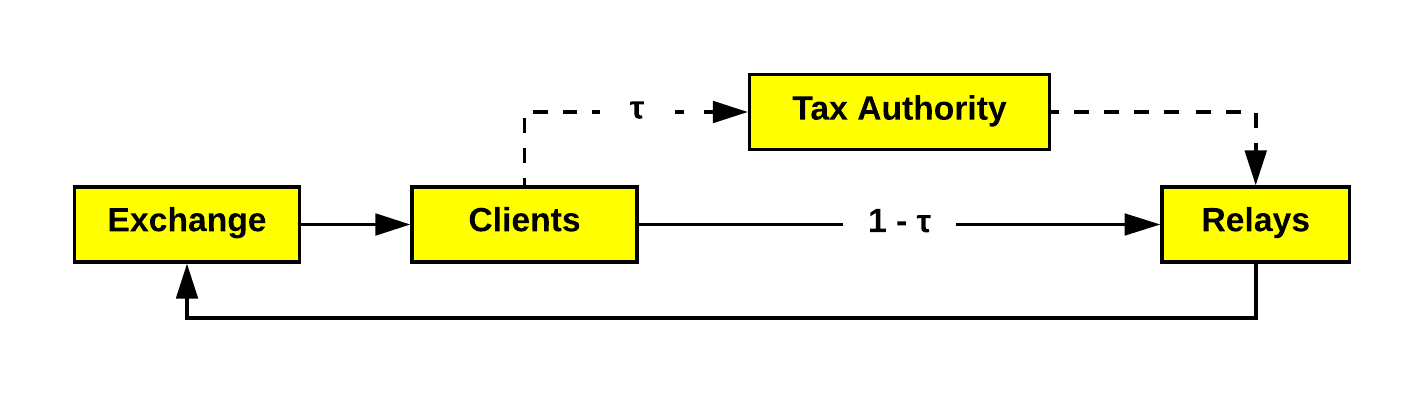
\includegraphics[trim={0.5cm, 0.5cm, 0.5cm, 0.5cm}, clip, scale=0.7]{images/economic_diagram.png}
%  \caption[Cash Flow]{Cash Flow --- movement of moneTor tokens through the
%    network. The value $\tau$ denotes the fraction of money that is collected
%    for taxation purposes.}
%  \label{fig:economic}
%\end{figure}

Given the delicate nature of this research area, a key motivation in
the design of our scheme is to explicitly accommodate some of the more
consequential economic considerations. For instance, to ensure that
tokens maintain real-world value, the Tor Project has two 
choices. One option is to reserve total monetary policy, allowing
moneTor tokens to mirror some external value signal such as the USD or
the Euro. Alternatively, by making use of such inter-ledger protocols~\cite{back2014enabling}~\cite{poon2017plasma}, tokens can act
as wrapper for an external cryptocurrency such as Bitcoin or
Ethereum. This choice represents a tradeoff between financial
stability and responsibility and our technical scheme allows for
either option.

The shape of the network that will emerge in a purely profit-seeking
environment may not perfectly correspond with the central goals of the
Tor Project: to advance human rights and freedoms. To this end, we
introduce a taxation element, enabling a tunable control mechanism
for The Tor Project to shape the topology of the network towards some
notion of desirable diversity and performance. Taxes in moneTor are
anonymously diverted into a shared global fund and eventually
redistributed to relays via a transparent policy, for instance, to
support areas where anonymity is needed but financial resources are
scarce. The exact content of such policy is an active subject of
research that is orthogonal to our paper.~\footnote{E.g.,
  Waterfilling~\cite{waterfilling-pets2017} argues for security by
  maximum diversity in endpoints of user paths, and
  TAPS~\cite{taps-ndss2017} argues for security by trust policies.}

The final considerationis the issue of price determination. While it
would be tempting to enlist some market-based mechanisms to set premium
bandwidth prices, any price differentiation between clients or relays inevitably
leaks more information. This leakage becomes more severe with higher granularity
payment options as adversaries begin to use price to link payment channels and
circuits. We therefore impose the constraint that all users should pay a single
uniform price for premium bandwidth at any time $t$. This price may be set
through a centralized calculation by the authorities or a more dynamical
consensus vote reached by the network.



%\subsection{Incentivized Conformity} In a decentralized network, there is no
%practical way to enforce standard behavior at each local node. We must therefore
%consider whether all nodes are rationally incentivized to obey the stipulated
%policies. For instance, we cannot guarantee that relays will actually confer
%premium bandwidth to paying users. Even though the relay has no particular
%reason to deviate, the client should periodically monitor her bandwidth and only
%make payments when they appear to be making a difference. The relationship
%between the client and relay can then be modeled as a game theoretic tit-for-tat
%dynamic within the immediate session. Over the long term, non-conforming relays
%might be blacklisted via Tor's existing reporting system.
%
%At the opposite end of the spectrum, relays might overly prioritize premium
%circuits while rejecting all traffic from unpaid users. They might also attempt
%to game the tax redistribution process to gain larger share of the proceeds. The
%bandwidth measurement authorities must anticipate such modes of deviation from
%the standard behavior to ensure that the risk for a relay to get blacklisted
%from the network is greater than the incremental gains it might attain from
%cheating. These attacks, while manageable, suggest that it would be prudent to
%limit the complexity of our economic policies until we can better study
%behavioral deviation dynamics in the live network.


\subsection{Ledger}

%The moneTor framework first requires a base layer payment protocol for users to
%anonymously and securely manage their funds.
In our payment design, we follow the Bitcoin paradigm in which all users
maintain full and exclusive control of their monetary wealth through use of
public key cryptography~\cite{nakamoto2008bitcoin}. However, unlike Bitcoin, it
is unnecessary for moneTor to rely on an inefficient decentralized consensus
mechanism. Since Tor already relies on a centralized set of authorities, we
simply introduce a new ledger authority role to maintain the global payment
state on a public tamper-evident database~\cite{crosby2009efficient}. To
maximize availability, this ledger may also be distributed across several
authorities with, for example, the architecture proposed by
RSCoin~\cite{danezis2015centrally}. This work focuses on payment protocol designs and evaluation. Therefore, we consider the investigation and choice of the right ledger technology as an independent problem out of scope of this paper.

%\op{Maybe add that RScoin might be a good ledger architecture on which our protocols rely?}

%%%
%  This part would either need more information or be removed to avoid reviewers to feel confused
%%%
%Structuring the ledger to understand
%blockchain-like semantics allows us to make use of recent developments in
%blockchain interoperability, allowing moneTor tokens to be pegged at a 1:1 ratio
%to a more popular cryptocurrency such as Bitcoin or
%Ethereum~\cite{back2014enabling, poon2017plasma}. The Plasma model in particular
%has many desirable properties. Under this setup, the moneTor ledger would act as
%a ``child chain'' that is coupled to the main Ethereum blockchain. This allows
%the external public blockchain to become the authority ledger of last resort in
%the event that the moneTor ledger goes offline. Effectively, honest users will
%always be able to make some claim to their funds so long as the Ethereum network
%is operational.
%Finally, moneTor requires anonymous payment procedures to allow users to make
%private low-frequency transactions. Potential candidates include Cryptonote,
%which makes use of stealth addresses and ring
%signatures~\cite{van2013cryptonote}, and Zerocash, which employs more expensive
%but more theoretically secure zero-knowledge proofs~\cite{sasson2014zerocash}.

\subsection{Payment Protocols Overview}
\label{sec:payment_overview}

In this section we specify formal protocols that comprise the payment
scheme. All protocols are either two or three party interactions between a
subset of the following roles: $C$ (client), $R$ (relay), $E$ (end user: either
a client or relay), $I$ (intermediary), and $L$ (ledger). All communications between end users and Intermediaries or the ledger are routed through Tor circuits.

The moneTor payment scheme is an extension of Bolt's three-party
bidirectional micropayment channels. In Bolt, multiple payments happens off-chain and cannot be linked together, even if the parties collide. Inspired from the Lightning Network~\cite{poon2016bitcoin}, payments can be routed through a third-party in a trustless fashion. In our design, we introduce an Intermediary relay which is only tasked to provide \emph{atomic} payment channel services between clients and relays and does not participate in routing user streams. These choices are made from the following benefits: 1) it escapes the naive setting whereby each Tor client maintains a micropayment channel with each
relay would incur an $O(n*m)$ cost with
respect to channel management complexity, with $n$ the number of Tor clients and $m$ the number of relays. By engineering an additional
intermediary layer, the complexity of moneTor channel connections is
reduced to $O(n+m)$; 2) CPU-intensive tasks are shifted by our protocol design to those intermediaries, allowing a payment system far more efficient than previous work in critical positions (i.e., relays, Tor authorities and clients). We detail it in related work Section~\ref{sec:related_work}; 3) the intermediaries can be incrementally deployed to match the right trade-off between performance of channel establishments and partition of premium users anonymity set (i.e., typically a premium user uses a same intermediary during a long time, we will see why later).
We adopt Bolt's nomenclature where
possible but adapt it to our concepts of ledgers, clients, and relays. The
following is brief outline of the prerequisite micropayment channel procedures
defined in Bolt. We refer the reader to the original paper for more detailed
specifications~\cite{green2017bolt}.

\begin{itemize}
\item \textbf{KeyGen}: Any party generates a cryptographic keypair
\item \textbf{Init-E}: $E$ initializes half of a micropayment channel by
  escrowing funds on $L$
\item \textbf{Init-I}: $I$ initializes half of a micropayment channel by
  escrowing funds on $L$
\item \textbf{Establish}: $E$ and $I$ interact to establish a new micropayment
  channel from their respective halves
\item \textbf{Pay}: $C$ interacts with $I$ and $R$ to send a single micropayment to $R$
\item \textbf{Refund}: $E$ closes a channel on $L$ and makes a claim on
  the escrowed funds.
\item \textbf{Refute}: $I$ closes a channel on $L$ and makes a claim on
  the escrowed funds.
\item \textbf{Resolve}: $L$ determines the final balance of funds awarded to
  each party.
\end{itemize}

While anonymous micropayment channels present a tremendous advance for many
applications, the relatively heavy cryptography ($37-100\ ms$) and communication
(7 message legs) is a prohibitive expense for Tor relay payments. Indeed, using Bolt would not permit a fair exchange (i.e., a high payment rate) between a client and a relay since we would need several \textit{RTTs} to complete a payment while ``consuming'' premium bandwidth and not being able to keep up with payments (in Bolt, the previous Pay needs to be finished to start the next one). Moreover, in terms of CPU overhead, it is also desirable to keep the
barrier of entry low for smaller relay operators. To overcome these
concerns, we present a new payment layer design enabling far more efficient
nanopayments that will satisfy our fair exchange problem and our overhead problem.

\textbf{moneTor} The moneTor construction makes use of the existing anonoymous
micropayment structure to facilitate \emph{locally transparent nanopayments}. In
this scheme, \emph{nanopayment channels} between clients and relays are established in place of a single
micropayment operation through an intermediary (Figure~\ref{fig:parties}). These lightweight channels allow the client to send $n$
number of unidirectional nanopayments to the relay. Each payment represents a
fixed value $\delta$, established at the start of the channel. The payments
themselves are \emph{locally transparent} in the sense that each nanopayment in
the same channel is trivially linked to each other (in contrast to previous works where several payments in the same circuit were needlessly unlinkable, details in Section~\ref{sec:related_work}). However, the nanopayment
channels themselves are unlinkable to other nanopayment channels and
micropayment operations. It is by design that this channel anonymity model fits
well with Tor's existing circuit framework in which one nanopayment channel is attached per circuit for each relay, and in which messages within circuits are
linkable with each other but the circuits themselves are not. In this sense, the
overarching motivation of our work is to relax the costly anonymity guarantees
provided by Bolt toward the design of a new set of protocols that have been
optimized for Tor. Note that the establishments and closures of nanopayment channels do not require the clients or relay to interact with the ledger, which offers a far more scalable design than previous works as we do not need to scale trusted or semi-trusted entities (only trustless intermediaries).

 We now briefly describe our new set of protocols.
\begin{figure}[h] \centering
  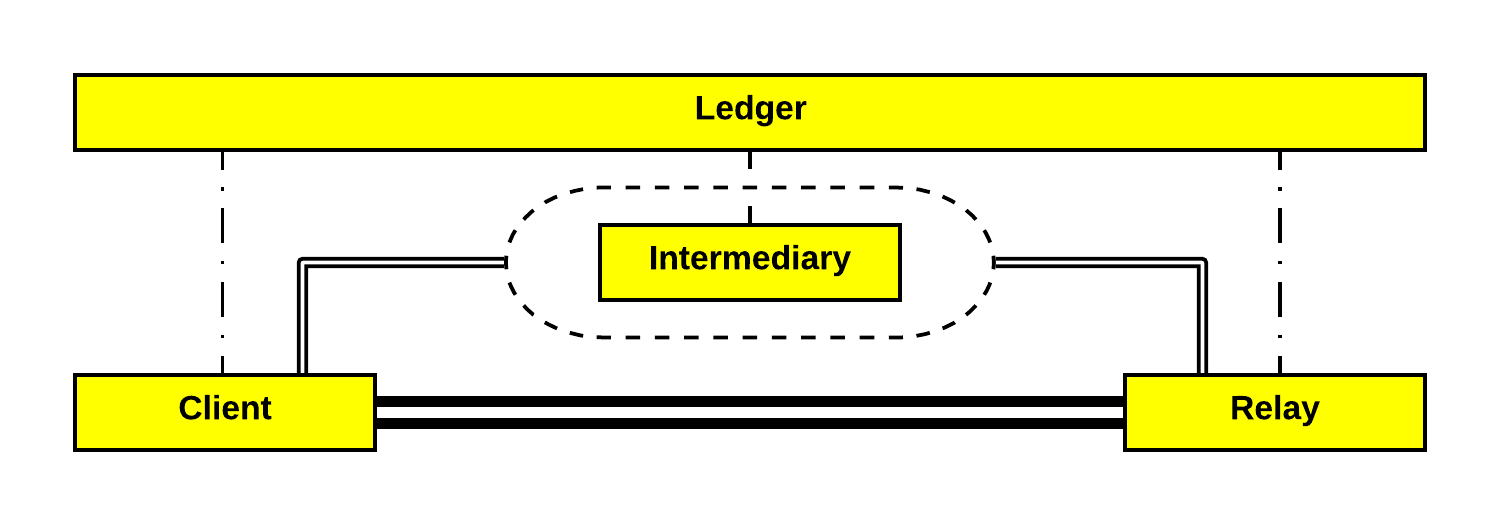
\includegraphics[trim={0.5cm, 0.5cm, 0.5cm, 0.5cm}, clip, scale=0.6]{images/party_diagram.png}
  \caption[Payment Roles]{Payment Roles --- Dashed lines represent periodic
    transactions (rare), thin double lines indicate micropayment channels (used at the beginning and end of circuits lifetime), and thick
    double lines indicate a nanopayment channel (handling nanopayments during the lifetime of the circuit). The dashed outline around the
    intermediary represents a notion of payment anonymity for the end users. Connections to the ledger and to the intermediary are protected by an internal Tor circuit.}
  \label{fig:parties}
\end{figure}
Any two parties $C$ and $R$ can construct a nanopayment channel once both have
completed Bolt $Establish$ with a common intermediary $I$. We define the following
set of protocols needed to manage nanopayments.

\begin{itemize}
\item \textbf{Nano-Setup} $C$ and $I$ interact to prepare an incomplete half of
  a nanopayment channel on top of their existing micropayment channel.
\item \textbf{Nano-Establish} $C$ sends her nanopayment channel information to
  $R$, who interacts with $I$ to complete the second half of the nanopayment
  channel on top of their own existing micropayment channel.
\item \textbf{Nano-Pay} $C$ sends a single nanopayment to $R$. This is
  repeatable for up to $n$ operations.
\item \textbf{Nano-Close-R} $R$ closes his nanopayment channel with $I$.
\item \textbf{Nano-Close-C} $C$ closes her nanopayment channel with $I$. Note that
  this must happen after \emph{Nano-Close-R}.
\end{itemize}

We also specify the following modified channel conflict resolution procedures to
ensure secure closure properties for the nanopayment scheme. Note that a malicious party can force a closure (i.e., abort), but will not be able to steal anything thanks to the dispute resolution on the ledger. It is important to note that the following algorithms run only in case of misbehaviour.

\begin{itemize}
\item \textbf{Nano-Refund} $E$ closes the channel on $L$.
\item \textbf{Nano-Refute} $I$ closes the channel on $L$.
\item \textbf{Nano-Resolve} $L$ makes final determination on both micropayment and
  outstanding nanopayment balances.
\end{itemize}

The core of our nanopayment scheme is inspired by the classic \emph{Payword}
two-party micropayment scheme in which payments are encoded by successively
revealed preimages in a precomputed hash chain~\cite{rivest1996payword}. 
%Hash
%chains are perhaps the most efficient known method for representing payments. In
%contrast to the expensive zero-knowledge proofs and signatures involved in
%anonymous micropayments, hash chain payments can be computed on the order of
%millions of hashes per second and conferred with a single 256 bit message, or
%one Tor cell.

The challenge in this construction is to securely integrate the hash chain
concept into an existing three-party anonymous micropayment channel setup such
that all parties maintain secure cryptographic ownership of their funds at all
steps. At the same time, we must ensure that no deanonymizing information is
leaked outside of the nanopayment channel context. We proceed to present a
concrete scheme which incurs an overhead penalty of approximately two
micropayment operations per nanopayment channel, one at the beginning and one at
the end of the channel life cycle.

\subsection{Nanopayment Protocols Details}
\label{sec:nanopaymentdetails}
In this section, we provide a summarized intuition for the basic steps in the
payment protocol. A more formal treatment of the steps are provided in
Appendix~\ref{sec:algorithms} with algorithmic details. Security considerations
are detailed next in Section~\ref{subsec:paysecurity} and formally
described in Appendix~\ref{sec:proof}.


\textbf{Nano-Setup} At the start of this protocol, $C$ has access to a
micropayment wallet $w$ obtained from Bolt's \textbf{Establish} that enables her to operate her micropayment channel
with $I$ as well as a refund token $rt$ that entitles her to claim her current
funds on $L$ should $I$ misbehave or go offline. To construct a nanopayment
channel, $C$ first generates an array of values $hc$ of length $n$ where
$hc_i = H(hc_{i+1})$ and $hc_n$ is a random number. The root of the hash chain
$hc_0$ is used to create a globally unique nanopayment token $nT$ that encodes
the public parameters of the channel including the length $n$ and the
per-payment value $\delta$. $C$ sends $I$ a commitment to a fresh nanopayment
channel parametrized by $nT$ along with a zero-knowledge proof of the following
statements:

\begin{enumerate}
\item The nanopayment wallet $nw$ is well-formed from $w$
\item $C$ has ownership of a micropayment channel containing at least $n *
  \delta$ funds.
\end{enumerate}

$I$ verifies these messages and supplies $C$ with a new signed refund token
$nrt$ that entitles $C$ to cash out the full balance of the micropayment channel.
%%%
%wut? Any nanopayments to L?
% This would be analagous to transation fees in Bitcoin as way to compensate
% ledges strictly for their computational consts... I guess we don't have
% to explicitly mention this if you don't want.
%%%
%along with any nanopayments to $L$.
$C$, now protected against misbehavior by
$I$, agrees to send a revocation token $\sigma_w$, which revokes her right to
use $w$ or $rt$. $I$ is now protected against double spending by $C$ and can
safely inform $C$ that the nanopayment channel has been set up successfully.

\textbf{Nano-Establish} At this point, $C$ sends $R$ the same $nT$ token used to
setup the channel with $I$. $R$ uses the token to initiate her end of the
nanopayment channel with $I$ by executing essentially the same procedure that
$C$ used in \emph{Nano-Setup}. The nanopayment channel is now fully established and
ready to be used. A key observation is that both ends of the channel ($C$-$I$
and $R$-$I$) are rooted at the same hash chain root $hc_0$.

\textbf{Nano-Pay} To make the next $i^{th}$ payment, $C$ simply sends the next
hash preimage $hc_i$ to $R$. Knowledge of this preimage $hc_i$ is sufficient for
$R$ to prove possession of a nanopayment. At any given time, $R$ can broadcast
the tuple ($nrt$, $hc_i$) to $L$ to prove ownership of the correct balance of
funds. Notice that this action simultaneously reveals $hc_i$ to $I$, who can
then claim an equivalent value of funds from $C$. As a result, the
scheme satisfies a correct-by-construction property of \emph{atomicity}
whereby both legs of the protocol are finalized at the same time.

\textbf{Nano-Close} After some number of payments $k < n$ has transpired and $C$
wants to close the Tor circuit, both $C$ and $R$ will generally prefer to close
their nanopayment channels through $I$. In this process, the $R$-$I$ leg must be
closed before the $C$-$I$ leg. This is due to the unidirectional nature of
nanopayment channels. Since payments are flowing form $C$ to $R$, $I$ must first
determine its debt to $R$ in order to know how much it can claim from $C$.

$R$ first sends to $I$ a commitment to a new micropayment wallet $w'$ and a
zero-knowledge proof of the following statements:

\begin{enumerate}
\item $w'$ is well-formed from $w$ ($w$ was either created by Bolt's establish phase or by a previous moneTor Nano-Close)
\item The balance of $w'$ is equal to the sum of the balance from the previous
  wallet $w$ and $\delta * k$
\end{enumerate}

Once verified, $I$ issues a refund token $rt'$ on the new funds. $R$ agrees to
invalidate the nanopayment channel by issuing a revocation token $\sigma_{nw}$
to $I$. $I$ and $R$ proceed to create a blind signature on $w'$ thus validating
the wallet for future use.

Once $I$ has closed his nanopayment channel leg with $R$, $I$ and $C$ are free
to complete the exact same close protocol. All parties are now reverted to the
original state they occupied prior to \emph{Nano-Setup} save for a securely updated
balance.

\textbf{Nano-Refund, Nano-Refute, Nano-Resolve} Honest parties will not typically
close active nanopayment channels on the ledger, opting instead to run Bolt
micropayment closure procedures when they wish to cash out. However, in the
event of malicious behavior or premature abortion, \emph{Nano-Refund} and
\emph{Nano-Refute} outlines procedures for $E$ and $I$ to withdraw funds on the
ledger at any given step with the latest payment information. After a set amount
of time allowing for the counterparty to reciprocate, the ledger runs
\emph{Nano-Resolve} to make a final publicly verifiable determination on the final
balance. Correct execution of these procedures allow all honest parties to
retain their funds in some cases and obtain the full balance of the malicious
party's escrowed funds in others.

\subsection{Tax Integration}

The zero-knowledge setup allows an elegant way to anonymously handle the
tax collection policy. Thus far, we have
treated the nanopayment value $\delta$ as symmetric for both the client and
relay leg. In practice, it requires only a trivial modification to specify
separate values of $\delta_C$ and $\delta_R$ such that the following equality is
satisfied.
\begin{equation}
  \delta_C - \delta_R = tax + fee
  \label{eq:payment}
\end{equation}
Here, $tax$ is the portion of every payment that is redirected to the Tor tax
authority while $fee$ represents compensation for $I$'s services. $I$ gradually
accumulates these overhead charges in his balance over the course of running
many nanopayment channels. When it is time for $I$ to cash out the full
micropayment channel, $L$ simply divides the funds between the $I$ and the tax
authority. Note that this does \emph{not} mean that $L$ can arbitrarily control
money as this process is well-defined in setup of the network protocol.

\subsection{Integration in Tor circuits}
Up to this point, we have described payments that occur between a single client
and a single relay. In practice, it is typical for each client to maintain a
handful of concurrently active circuits,\footnote{For instance, the popular Tor
  Browser user application typically does not share circuits with streams targeting a different destination address unless those streams come from the same SOCKS connection.}  each of
which requires three streams of payments to the guard, middle, and exit
relays. These channels must be actively managed to optimize computational
overhead as well as money flow. Furthermore, connections between the client and
the guard relay are transparent and persistent across the timescale of several
months. We optimize toward this setup by enabling transparent and direct payment
channels between the client and guard, considerably reducing the network
overhead costs.

\subsection{Payment Security and Anonymity}
\label{subsec:paysecurity}
Our security model must account for both privacy and payment security. The
privacy threat model is derived from the local active adversary paradigm
ubiquitously found in Tor research~\cite{dingledine2004tor}. Like all cells in
Tor, Nanopayment messages are locally linkable by relays participating in the
circuit. However, since each circuit is only ever associated with one anonymous
micropayment channel at any given time, we can guarantee that relays and
intermediaries cannot link two nanopayment channels with the same user. Formal
definitions and proofs are provided in Appendix~\ref{sec:proof} for the following theorem:

\begin{theorem}
The nanopayment channel scheme satisfies the properties of anonymity (\ref{def:anon1}, \ref{def:anon2})
 and security (\ref{def:balance}) under the restriction that the adversary does not abort before Nano-Close finished, the restrictions that at most one nanopayment channel can be open per micropayment channel, the assumptions that the commitment scheme is secure, the zero-knowledge system is simulation extractable and zero-knowledge, and the hash function used to create the hashchain and verify the preimage during the Nano-Pay is a cryptographic hash function.

\end{theorem}

Any communication in
our tripartite nanopayment protocol are protected by Tor circuits. Hence,
relationship between client to intermediary, client to ledger, relay to
intermediary and relay to ledger are themselves anonymized by Tor circuits. If
some party aborts, which induce a dispute on the ledger, the relationship
between the client and his relays is protected by the various Tor circuits built
to resolve the dispute with the ledger.

Informally, we claim the following anonymity guarantees relative to unmodified Tor:

\begin{enumerate}
\item Additional parties needed to operate the moneTor system (i.e. ledgers and
  intermediaries) cannot extract any more information about a given client than
  any middle relay.
\item Excluding side channels, circuits do not leak any more information than
  the single bit needed to differentiate premium and nonpremium users.
%\item There is no more anonymity set partitioning than a partition of premium Tor users and non-premium Tor users.
  % ^^ this seems partially redundant with point 2, no? 2 implicitly says that (A) the anonymity set
  % is partiioned and (B) we know that people in the premium group somehow care
  % more about their traffic speed. Maybe we can break it up along those lines
  % if you want to be more explict
\end{enumerate}

Our current payment protocols expose a subtle passive attack by $I$ which our security model does not capture. By examining
the final number of payments made on each channel in conjunction with the
globally fixed nanopayment cost, $I$ may potentially link all of $C$'s
nanopayment channels\footnote{This attack is best illustrated with a trivial
  example. Suppose that $I$ facilitates a number of nanopayment channels with
  the following number of payments, each of which is known to represent one unit
  of money: $[58, 839, 356, 881, 23, 89, 561]$ Now that $C$ closes her
  micropayment channel and terminates with exactly 404 units of money. Once the
  micropayment channel is closed, $I$ must necessary gain knowledge of the final
  balance of funds and can easily link the first and third nanopayment channels
  as belonging to the same $C$.}. To mitigate this vulnerability, we stipulate
that $C$ must make at least one micropayment, which has a monetary value hidden
from $I$, before closing a micropayment channel. We expect that this
micropayment should contain a random value not greater than the channel escrow
maximum value as stated in the Tor consensus and may be made to another account
owned by $C$.

Our threat model for payment security is similar to those found in prior works
in blockchain micropayment channels~\cite{poon2016bitcoin}. In such models, the
user is protected from malicious intermediaries by the ability to prove
misbehavior to a global ledger. Our protocols also guarantee that the client would not be claimed more money than initially agreed (Balance property \ref{def:balance}).
%
%The security of the ledger will be subject to
%the guarantees made by the cryptocurrency interface~\cite{back2014enabling,
%  poon2017plasma}. This is in direct contrast to prior Chaumian e-cash proposals
%that employ the \emph{honest but curious} model for the central bank in which
%banks have full control over user funds. Indeed, this is the basis for the
%difference in terminology between prior \emph{central banks} and the moneTor
%\emph{ledger}.

%An intermediary however, is able to observe any nanopayment channel establishment and closure linked to a particular micro payment channel. Because each nanopayment channel matches a particular Tor circuit, it can match the opening/closure timing of nano channels to track the activity of an anonymous user through time. User's activity may leak some information about the user itself or the user's behaviour (e.g., the timezone). Considering such side-channels is out-of-scope of this paper, however our moneTor design would make inefficient such attack if users open micro-channels with multiple intermediaries and hide their behaviour with a random use of the set of micro-channels they have opened. This would however increase the amount of escrowed fund needed.

%%% Local Variables:
%%% mode: latex
%%% TeX-master: "../main"
%%% End:
